\chapter{Preparación para el trabajo y secuencia de tareas}\label{ch:preparation}

\section{Preparar el vehículo}
Siga la secuencia siguiente al sustituir el cuadro de fábrica por un tablero Digifiz:
\begin{enumerate}
    \item Retire las molduras plásticas que cubren los pedales y la parte inferior del tablero para dejar al descubierto el cuadro original.
    \item Desconecte la batería del vehículo.
    \item Desenchufe el mazo de cables del cuadro de instrumentos de fábrica.
    \item Desacople el cable mecánico del velocímetro, si está presente.
    \item Desatornille el cuadro de sus soportes y extráigalo con cuidado del vehículo.
    \item Guíe los mazos de sensores de temperatura y velocidad suministrados según sea necesario.
    \item Instale el tablero Digifiz en las guías del soporte y fíjelo con tornillos.
    \item Para \ReplicaNextLong{}, instale los sensores MFA de Volkswagen (o equivalentes) y lleve sus conductores hasta los conectores CE~1/CE~2.
    \item En los modelos \texttt{GACS}/\texttt{GARS}/\texttt{DARS}/\texttt{DACS}, conecte manualmente los cables etiquetados \texttt{MFA\_MODE}, \texttt{MFA\_RESET}, \texttt{MFA\_BLOCK} y freno de mano si el mazo del vehículo carece de estos contactos. La segunda generación \ReplicaNextShort{} conecta estas señales internamente por defecto.
    \item Conecte los mazos al cuadro.
    \item Monte el sensor de velocidad electrónico o vuelva a conectar el cable mecánico.
    \item Reinstale las molduras del tablero y la cubierta de los pedales en orden inverso.
\end{enumerate}

\section{Operación del tablero}
\begin{itemize}
    \item El cuadro se enciende automáticamente con el contacto. El interruptor de luces de posición controla la retroiluminación.
    \item Al inicio se ilumina toda la escala de velocidad mientras el autodiagnóstico estabiliza el modelo de RPM; la pantalla se estabiliza posteriormente en el régimen de ralentí actual.
    \item Una vez que el vehículo comienza a moverse, el sistema informa los parámetros descritos en \Cref{ch:technical-specs}.
\end{itemize}

\subsection{Funciones de la MFA}
Hay seis páginas MFA disponibles:
\begin{enumerate}
    \item Tiempo de funcionamiento diario.
    \item Distancia del trayecto.
    \item Consumo de combustible (no implementado en la primera revisión de Replica).
    \item Velocidad media (mostrada como el valor multiplicado por diez).
    \item Temperatura del aceite del motor (requiere mazo externo).
    \item Temperatura ambiente (requiere mazo externo).
\end{enumerate}
En los cuadros \ReplicaGenOneShort{} un punto táctil capacitivo detrás del emblema VW recorre las páginas; \ReplicaNextShort{} utiliza un interruptor externo en la columna de dirección. Las duraciones de pulsación se comportan de la siguiente manera:
\begin{itemize}
    \item Pulsación corta (\(<1\)~s): avanza a la siguiente función MFA.
    \item Pulsación media (1--3~s cuando no hay interruptor en la columna): alterna entre bloques de memoria MFA; el cambio se indica en pantalla.
    \item Pulsación larga (3--7~s): reinicia la función MFA activa (afecta al consumo, distancia del viaje, tiempo transcurrido y velocidad media).
\end{itemize}

\subsection{Distribución de retroiluminación e indicadores}
El cuadro \ReplicaGenOneShort{} ofrece un ajuste manual de brillo sobre el interruptor de luces de estacionamiento; \ReplicaNextShort{} confía en el brillo automático gobernado por un fotodiodo. Se pueden configurar anulaciones manuales mediante las interfaces de mantenimiento descritas en \Cref{ch:replica-setup,ch:replica-next-setup}.

La disposición del bloque horizontal de testigos y la leyenda en pantalla se muestran en \autoref{fig:indicator-layout}.

\begin{figure}[htbp]
    \centering
    \begin{subfigure}{0.48\textwidth}
        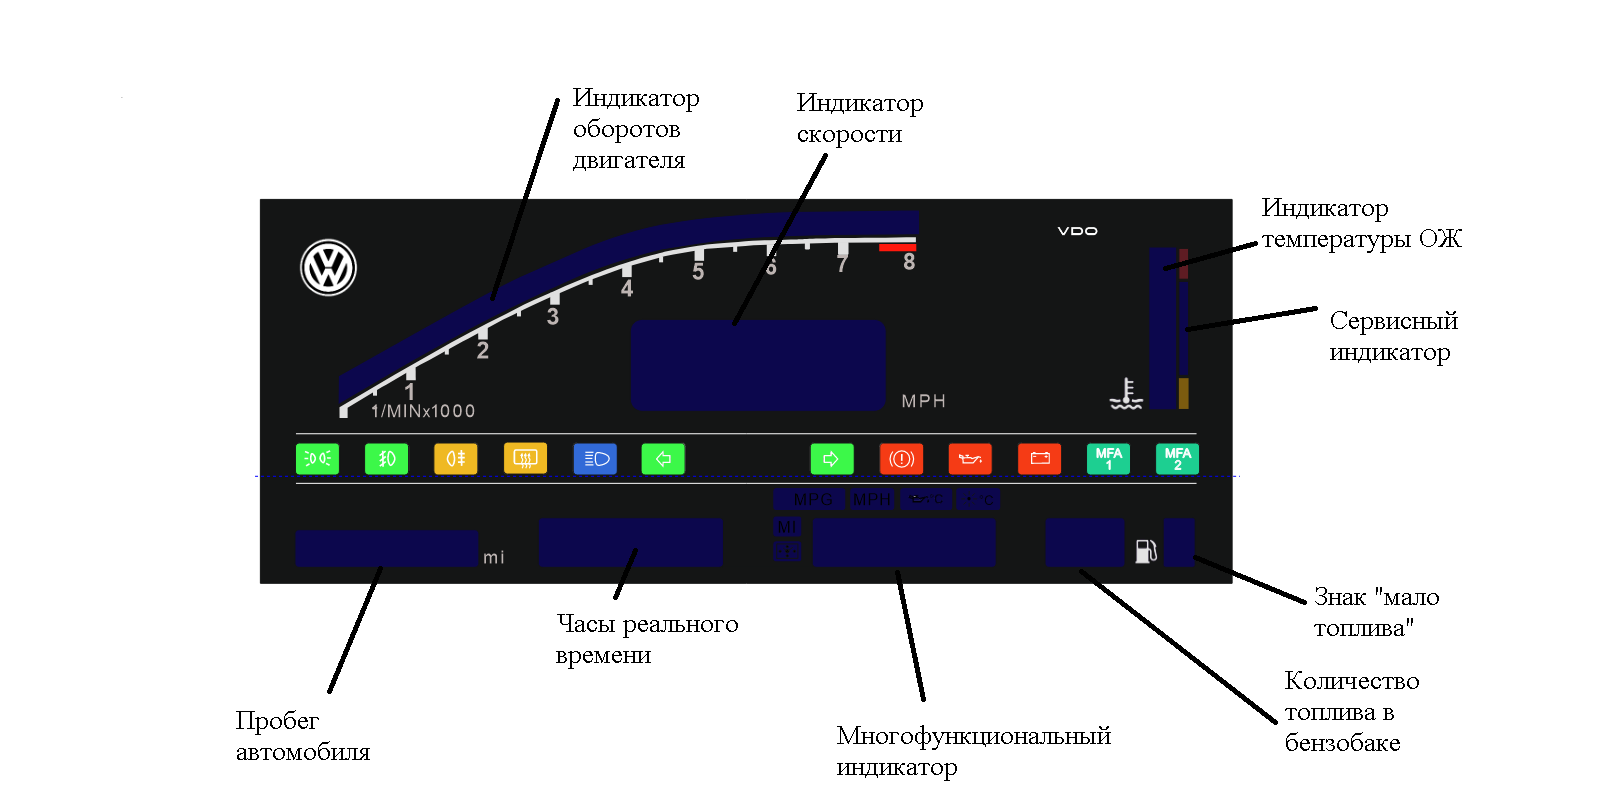
\includegraphics[width=\linewidth]{digifiz_manual/image017.png}
        \caption{Disposición de testigos mostrada durante la autocomprobación de encendido.}
    \end{subfigure}\hfill
    \begin{subfigure}{0.48\textwidth}
        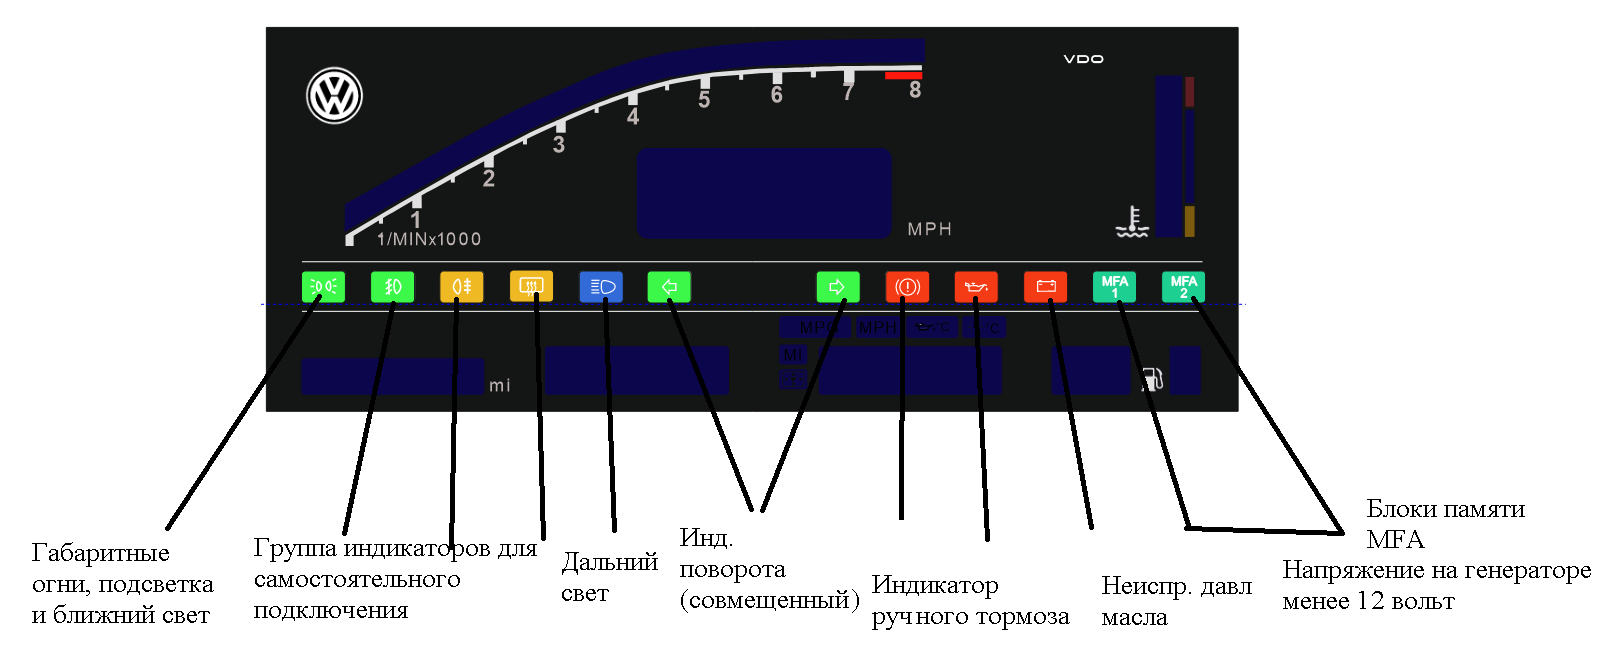
\includegraphics[width=\linewidth]{digifiz_manual/image018.png}
        \caption{Leyenda del grupo horizontal de indicadores.}
    \end{subfigure}
    \caption{Esquema de indicación del cuadro de instrumentos.}
    \label{fig:indicator-layout}
\end{figure}

\subsection{Interfaces de configuración}
\begin{itemize}
    \item Las unidades \ReplicaGenOne{} clásicas incluyen un módulo Bluetooth 2.0 (o compatible con BLE). Instale la aplicación \emph{Serial Bluetooth Terminal} desde Google Play, empareje con el cuadro y ejecute comandos directamente desde la vista de terminal. Los dispositivos Apple iOS no pueden conectarse a este módulo.
    \item \ReplicaNextShort{} expone un punto de acceso Wi-Fi integrado y un portal de configuración descrito en \Cref{ch:replica-next-setup}. Desactive los datos móviles durante la conexión para asegurarse de que el portal cautivo cargue correctamente.
\end{itemize}
Ambas generaciones pueden alimentarse y configurarse en banco utilizando la interfaz de programación USBasp.
